\tolerance=1
\emergencystretch=\maxdimen
\hyphenpenalty=10000
\hbadness=10000


\documentclass[20]{beamer}

\mode<presentation>
{
  \usetheme{NYU}  
  \usecolortheme{default} % or try albatross, beaver, crane, ...
  \usefonttheme{serif}  % or try serif, structurebold, ...
  \setbeamertemplate{navigation symbols}{}
  \setbeamertemplate{caption}[numbered]
} 

\usepackage[english]{babel}
\usepackage[utf8x]{inputenc}
\usepackage[T1]{fontenc}
\usepackage{tikz}
\usepackage{venndiagram}
\usepackage{amsmath}
\usepackage{graphicx}
\usepackage[colorinlistoftodos]{todonotes}
\usepackage[document]{ragged2e}
\usepackage{lipsum}
\usepackage{algorithm2e}
\usepackage{ragged2e}


\title[University of Connecticut ARE Seminars]{Using network analysis to understand the dynamics of the organic dairy sector since the inception of the 2002 organic regulation}
\author{Carolyn Dimitri, Juan C. S. Herrera}
\date{March 8 2019}
\titlegraphic{\hfill\includegraphics[height=1.5cm]{nyu_stacked_color}}

\expandafter\def\expandafter\insertshorttitle\expandafter{%
  \insertshorttitle\hfill%
  \insertframenumber\,/\,\inserttotalframenumber}


\begin{document}

\begin{frame}
  \titlepage
\end{frame}

% Uncomment these lines for an automatically generated outline.
%\begin{frame}{Outline}
%\tableofcontents
%\end{frame}

\begin{frame}{1. Introduction: What is Network Analysis ?}
\justify
\textbf{Network analysis is a methodology to study interconnected systems \textit{(G)} represented by nodes \textit{(V)} and edges  \textit{(E)}}
\\ 
\[G = (V, E)\]

The \textbf{nodes} are a finite set of identifiable entities that can potentially take part in the relationship under study. The relationships between the nodes are represented by \textbf{edges}. The set of nodes and edges is defined as a \textbf{network} (Butts 2009, 414; Newman 2010)

\end{frame}


\begin{frame}{Introduction: Food Networks}
\textbf{Examples of Food Networks}
\\ 
\vspace{0mm}
\begin{itemize}
\item \textbf{Food Recipes:} 
\\Nodes: Ingredients, Recipe Titles, Preparation Techniques
\\Edges: Ingredients connected to recipe titles, ingredients connected to preparation techniques
\end{itemize}

\centerline{Network of Three Coffee Recipes}

\resizebox{!}{0.32\textwidth}{%
  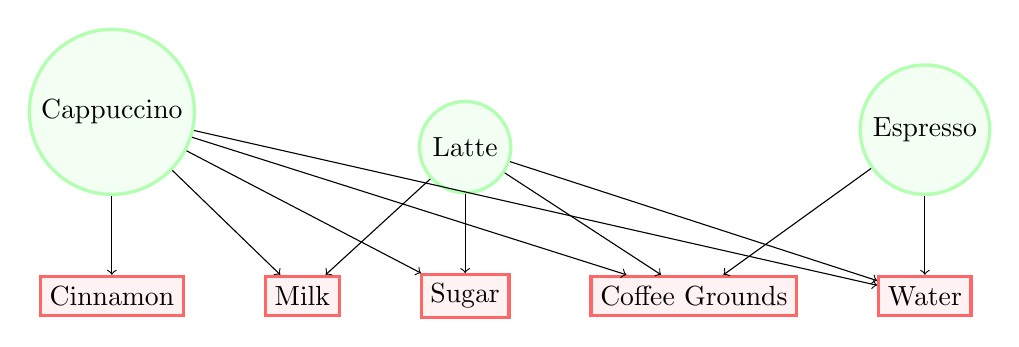
\begin{tikzpicture}
  [
  roundnode/.style={circle, draw=green!30, fill=green!5, very thick, minimum size=5mm},
  squarednode/.style={rectangle, draw=red!60, fill=red!5, very thick, minimum size=5mm},
  ]
  %Nodes
  \node[roundnode]      (Cappuccino)                          {Cappuccino};
  \node[squarednode]        (Cinnamon)        [below=of Cappuccino] {Cinnamon};
  \node[squarednode]        (Milk)            [right=of Cinnamon] {Milk};
  \node[squarednode]        (Sugar)           [right =of Milk] {Sugar};
  \node[squarednode]        (Coffee Grounds)  [right=of Sugar] {Coffee Grounds};
  \node[squarednode]        (Water)           [right=of Coffee Grounds] {Water};
  \node[roundnode]         (Latte)            [above=of Sugar]              {  Latte  };
  \node[roundnode]         (Espresso)         [above=of Water]              {Espresso};
  %Lines
  \draw[->] (Cappuccino) -- (Milk);
  \draw[->] (Cappuccino) -- (Cinnamon);
  \draw[->] (Cappuccino) -- (Sugar);
  \draw[->] (Cappuccino) -- (Coffee Grounds);
  \draw[->] (Cappuccino) -- (Water);

  \draw[->] (Latte) -- (Milk);
  \draw[->] (Latte) -- (Sugar);
  \draw[->] (Latte) -- (Coffee Grounds);
  \draw[->] (Latte) -- (Water);

  \draw[->] (Espresso) -- (Coffee Grounds);
  \draw[->] (Espresso) -- (Water);
  \end{tikzpicture}
}

\end{frame}


\begin{frame}{Introduction: Food Networks}
\textbf{Examples of Food Networks}
\\ 
\vspace{0mm}
\begin{itemize}
\item \textbf{Food Market}
\\Nodes: Food Market, Farms
\\Edges: Food transported from farm to food market
\end{itemize}
\vspace{2mm}
\centerline{Union Square Farmers Market - Farmers Network}
\vspace{0mm}
\centering
\resizebox{!}{0.32\textwidth}{%
  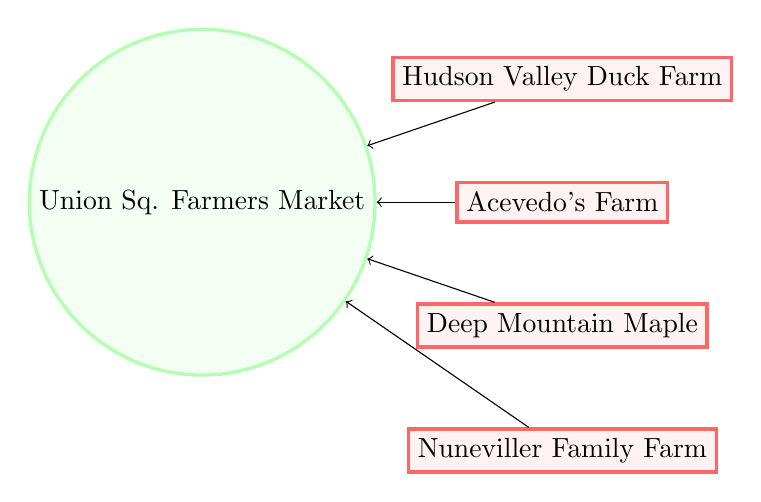
\begin{tikzpicture}
  [
  roundnode/.style={circle, draw=green!30, fill=green!5, very thick, minimum size=5mm},
  squarednode/.style={rectangle, draw=red!60, fill=red!5, very thick, minimum size=5mm},
  ]
  %Nodes
  \node[roundnode] (usq) {Union Sq. Farmers Market};
  \node[squarednode] (a) [right=of usq] {Acevedo's Farm};
  \node[squarednode] (b) [below=of a] {Deep Mountain Maple};
  \node[squarednode] (c) [above=of a] {Hudson Valley Duck Farm};
  \node[squarednode] (d) [below=of b] {Nuneviller Family Farm};
  %Lines
  \draw[->] (a) -- (usq);
  \draw[->] (b) -- (usq);
  \draw[->] (c) -- (usq);
  \draw[->] (d) -- (usq);
  \end{tikzpicture}
}


\end{frame}



\begin{frame}{Introduction: Food Networks}
\textbf{Examples of Food Networks}
\\ 
\vspace{0mm}
\begin{itemize}
\item \textbf{International Food Trade}
\\Nodes: Countries
\\Edges: Food products being exported and imported
\end{itemize}

\vspace{0mm}
\centerline{Network of Food Trade Between the USA and Canada }
\vspace{2mm}
\centering
\resizebox{!}{0.45\textwidth}{%
  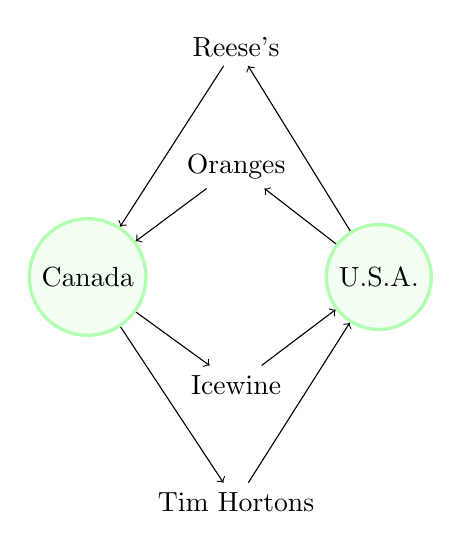
\begin{tikzpicture}
  [
  roundnode/.style={circle, draw=green!30, fill=green!5, very thick, minimum size=1mm},
  squarednode/.style={rectangle, draw=red!60, fill=red!5, very thin, minimum size=1mm},
  ]
  %Nodes
  \node[roundnode] (ca) {Canada};
  \node (x) [right=of ca] {};
  \node[roundnode] (cb) [right=of x] {U.S.A.};
  
  \node  (a) [below=of x] {Icewine};
  \node  (b) [below=of a] {Tim Hortons};
  \node (c) [above=of x] {Oranges};
  \node  (d) [above=of c] {Reese's};


  %Lines
  \draw[->] (ca) -- (a);
  \draw[->] (ca) -- (b);
  \draw[->] (a)  -- (cb);
  \draw[->] (b)  -- (cb);
  
  \draw[->] (cb) -- (c);
  \draw[->] (cb) -- (d);
  \draw[->] (c)  -- (ca);
  \draw[->] (d)  -- (ca);
  
  \end{tikzpicture}
}


\end{frame}



\begin{frame}{Introduction: Food Networks}
\textbf{Dissertation Title: Dynamic and Interconnected: Three essays on food networks with applications to food consumption and production. }
\\ 
\vspace{5mm}
\begin{itemize}
\item \textbf{Paper 1:} The Contribution of Network Analysis to the Study of Food Recipes. A Literature Review
\item \textbf{Paper 2: A Network Analysis of Organic Dairy in the United States of America, 2002-2015} 
\item \textbf{Paper 3:} {The Dynamics of Food Recipes: 6,000 Recipes Over 40 years. Colombia, 1977-2017}
\end{itemize}
\end{frame}


\begin{frame}{A Network Analysis of Organic Dairy in the United States of America, 2002-2015}
\textbf{Motivation}
\\ 
\begin{itemize}
\item Given that organic dairy farming is more profitable than conventional dairy farming, why has been the adoption of organic dairy farming slow in the USA?
\item  What is the logic behind choosing a geographical location to start an organic dairy farming operation?
\item  Can networks partially explain the geographic location of organic dairy farming in the USA?
\end{itemize}
\end{frame}


\begin{frame}{A Network Analysis of Organic Dairy in the United States of America, 2002-2015}
\textbf{Data: United States Department of Agriculture. Organic Integrity Database. June 8 2017}
\\ 
\begin{itemize}
\item Every organic operation is recorded in this database that is open to the public
\item The database contains information starting from 2002 when the National Organic Standards became law.
\item Each operation includes an address
\end{itemize}
\end{frame}


\begin{frame}{A Network Analysis of Organic Dairy in the United States of America, 2002-2015}
\textbf{Methodology}
\\ 
\begin{itemize}
\item 1. Get GPS Coordinates for each address representing an organic dairy production facility. \\ Operation name + address + state --> Google Maps --> GPS
\item 2. Infer Networks
\item 3. Use Network Analysis to study the simulated networks 
\end{itemize}
\end{frame}


\begin{frame}{A Network Analysis of Organic Dairy in the United States of America, 2002-2015}
\vspace{-1mm}
\begin{algorithm}[H]
\SetAlgoLined
\KwResult{280 Networks: 2002 - 2015, 20 Inferred networks per year.}
\While{t = 2002 to 2015 (1 year increments)}{
  \While{p = 5 to 100 (5\%\ increments)}{
    \eIf{$t$ = 2002}{
     - For each GPS coordinate create a 50 mile radius\;
     - Connect to other coordinates belonging to $t$ that are inside the radius with probability $p$;}{If $t$ > 2002 and t <= 2015 \textbf{then}\\
     - For each GPS coordinate create a 50 mile radius\;
     - Connect to other coordinates inside the radius that belong to $t <= t$ with probability $p$;}
     }
   }
\end{algorithm}
\end{frame}



\foreach \x in {0,1,2,3,4,5,6,7,8,9,10,11,12,13}
 {
  \begin{frame}{Geographic Location Of Organic Dairy Farmers in the USA}
   \begin{figure}
   \vspace{-1mm}
   \includegraphics[width=0.8\textwidth]{output-\x.png}
   \end{figure}
   \end{frame}
}


\begin{frame}{A Network Analysis of Organic Dairy in the United States of America, 2002-2015}
\textbf{From GPS Coordinates to Networks}

\includegraphics[width=0.5\textwidth]{output-0.png}%
\includegraphics[width=0.5\textwidth]{2002.png}
\vspace{-5mm}
To maintain the relevance of closer connections we use the standardized inverse from 0 to 1 for the weight of the edges. A 50 mile distance is now almost 0 and 0 mile distance is now almost 1.
\end{frame}


\foreach \x in {2002,2005,2010,2015}
 {
  \begin{frame}{A Network Analysis of Organic Dairy in the United States of America, 2002-2015}
   \begin{figure}
   \vspace{-1mm}
   \includegraphics[width=0.7\textwidth]{\x.png}
   \end{figure}
   \end{frame}
 }



\begin{frame}{A Network Analysis of Organic Dairy in the United States of America, 2002-2015}
\textbf{Network Analysis}
\\ 
\begin{itemize}
\item 1. Average separation over time
\item 2. Clustering coefficient
\item 3. Relative size of the largest cluster
\item 4. Average degree
\end{itemize}
\end{frame}


\begin{frame}{A Network Analysis of Organic Dairy in the United States of America, 2002-2015}
\begin{figure}
   \vspace{-1mm}
   \includegraphics[width=0.5\textwidth]{av_separation.png}
\end{figure}
\vspace{-5mm}
\begin{itemize}
\item Overall decrease in the number of connections that one farmer needs to go through to connect with another (Similar to 6 degrees of separation) 
\item Information moves faster between farmers
\item Smaller degrees of separation reflect a more cohesive network
\item Disconnected network. We use an inverse standardized proxy

\end{itemize}
\end{frame}


\begin{frame}{A Network Analysis of Organic Dairy in the United States of America, 2002-2015}
\begin{figure}
   \vspace{-1mm}
   \includegraphics[width=0.5\textwidth]{clustering_coefficient.png}
\end{figure}
\vspace{-5mm}
\begin{itemize}
\item The clustering coefficient measures the average probability, over the entire network, that the two closest nodes of a nearest neighbor node are connected 
\item  Communities tend to get more connected with their peers over time
\end{itemize}
\end{frame}


\begin{frame}{A Network Analysis of Organic Dairy in the United States of America, 2002-2015}
\begin{figure}
   \vspace{-1mm}
   \includegraphics[width=0.5\textwidth]{largest_cluster.png}
\end{figure}
\vspace{-5mm}
\begin{itemize}
\item The relative size of the largest cluster is an intuitive network statistic that is obtained by dividing the number of nodes that form the largest cluster (a group of connected nodes) by the number of total nodes in the network
\item In a network that becomes more connected over time, one expects this number to increase as the largest cluster gains more nodes 
\end{itemize}
\end{frame}


\begin{frame}{A Network Analysis of Organic Dairy in the United States of America, 2002-2015}
\begin{figure}
   \vspace{-1mm}
   \includegraphics[width=0.5\textwidth]{av_degree.png}
\end{figure}
\vspace{-5mm}
\begin{itemize}
\item The average degree is calculated by taking the mean of the number of connections of each node
\item A larger number means that each node is on average more connected. Given that the networks have a gps rationale we see evidence for clustering
\end{itemize}
\end{frame}

\begin{frame}{A Network Analysis of Organic Dairy in the United States of America, 2002-2015}
\textbf{Conclusions}
\begin{itemize}
\item The results evidence that the geo-location of new organic dairy producers reflects advantages from proximity to peers such as potentially benefiting from knowledge spillovers, know-how transmission, minimizing risk arising from uncertainty, and minimizing discrimination towards organic production. 
\item These effects may explain partially why the adoption of organic dairy production, which is more profitable has not been adopting in some regions of the country. 
\item Potential policies that seek to incentive organic dairy production should aim to strengthen the peer networks.  
\end{itemize}
\end{frame}


\begin{frame}{A Network Analysis of Organic Dairy in the United States of America, 2002-2015}
\textbf{Limitations and Future Research}
\begin{itemize}
\item Inferred networks.
\item 2008 marks an inflection point in our measures. With more data over more years we will probably see stronger conclusions
\item We have not included meteorological and land quality factors which may have an impact on our results

\vspace{4mm}
\item We are looking to include organic dairy handlers to strengthen our analysis
\item Possibly including consumers using supermarkets such as Whole Foods as an approximation
\end{itemize}
\end{frame}


\begin{frame}{A Network Analysis of Organic Dairy in the United States of America, 2002-2015}
\begin{center} 
  \textbf{THANK YOU} \\
  \vspace{4mm}
  \textbf{Juan C. S. Herrera} \\
  \vspace{4mm}
  \textbf{JSH501@NYU.EDU}
\end{center}

\end{frame}



\end{document}
